\documentclass[12pt,a4paper]{article}

% ─── Page Layout ───────────────────────────────────────────────────────────────
\usepackage[a4paper, margin=0.8in, headheight=14pt]{geometry}

% ─── Fonts (XeLaTeX) ───────────────────────────────────────────────────────────
\usepackage{fontspec}
\usepackage{unicode-math}
\setmainfont{TeX Gyre Pagella}
\setmonofont[Scale=0.88]{TeX Gyre Cursor}
\setmathfont{Latin Modern Math}

% ─── Packages ──────────────────────────────────────────────────────────────────
\usepackage{xcolor}
\usepackage{colortbl}
\usepackage{titlesec}
\usepackage{enumitem}
\usepackage{tabularx}
\usepackage{booktabs}
\usepackage{array}
\usepackage{amsmath}
\usepackage{tikz}
\usetikzlibrary{shapes.geometric, arrows.meta, positioning, calc, fit, decorations.pathreplacing}
\usepackage{tcolorbox}
\tcbuselibrary{skins, breakable}
\usepackage{hyperref}
\usepackage{fancyhdr}
\usepackage{graphicx}
\usepackage{microtype}
\hyphenpenalty=10000
\exhyphenpenalty=10000
\sloppy
\usepackage{caption}
\usepackage{setspace}
\usepackage{multirow}
\usepackage{tocloft}

% ─── Q&A helper ────────────────────────────────────────────────────────────────
\newcommand{\Q}[1]{\textbf{#1}\par\noindent\ignorespaces}

% ─── Colour Palette ────────────────────────────────────────────────────────────
\definecolor{myred}{RGB}{196,30,58}
\definecolor{mydark}{RGB}{30,30,50}
\definecolor{mygreen}{RGB}{14,120,80}
\definecolor{myteal}{RGB}{0,130,140}
\definecolor{myamber}{RGB}{180,100,0}
\definecolor{mypurple}{RGB}{100,30,160}
\definecolor{mygray}{RGB}{246,247,249}
\definecolor{mgframe}{RGB}{180,185,200}
\definecolor{watermark}{RGB}{145,150,170}
\definecolor{hdrred}{RGB}{250,232,235}
\definecolor{hdrgreen}{RGB}{220,244,233}
\definecolor{hdrteal}{RGB}{220,242,244}
\definecolor{hdramber}{RGB}{253,242,215}
\definecolor{hdrpurple}{RGB}{238,228,255}
\definecolor{hdrgray}{RGB}{238,240,245}
\definecolor{rowalt}{RGB}{250,251,253}

% ─── Section Formatting ────────────────────────────────────────────────────────
\titleformat{\section}
  {\large\bfseries\color{myred}}{\thesection.}{0.5em}{}
  [\vspace{1pt}{\color{myred}\rule{\linewidth}{0.8pt}}]
\titleformat{\subsection}
  {\normalsize\bfseries\color{myteal}}{\thesubsection}{0.5em}{}
\titlespacing*{\section}{0pt}{18pt}{7pt}
\titlespacing*{\subsection}{0pt}{11pt}{4pt}

% ─── Paragraph ─────────────────────────────────────────────────────────────────
\setlength{\parindent}{0pt}
\setlength{\parskip}{4pt}

% ─── TOC Styling ───────────────────────────────────────────────────────────────
\renewcommand{\cfttoctitlefont}{\large\bfseries\color{myred}}
\renewcommand{\cftaftertoctitle}{\par\noindent{\color{myred}\rule{\linewidth}{0.8pt}}}
\setlength{\cftbeforetoctitleskip}{0pt}
\setlength{\cftaftertoctitleskip}{6pt}
\renewcommand{\cftsecfont}{\normalsize\bfseries\color{mydark}}
\renewcommand{\cftsecpagefont}{\normalsize\bfseries\color{mydark}}
\renewcommand{\cftsecleader}{\cftdotfill{\cftdotsep}}
\setlength{\cftbeforesecskip}{7pt}
\renewcommand{\cftsubsecfont}{\small\color{mydark}}
\renewcommand{\cftsubsecpagefont}{\small\color{mydark}}
\setlength{\cftbeforesubsecskip}{3pt}
\setlength{\cftsubsecindent}{1.4em}

% ─── Table helpers ─────────────────────────────────────────────────────────────
\renewcommand{\arraystretch}{1.45}
\setlength{\tabcolsep}{6pt}
\arrayrulecolor{mydark}
\newcolumntype{B}[1]{>{\small\bfseries\raggedright\arraybackslash}m{#1}}
\newcolumntype{Y}{>{\small\raggedright\arraybackslash}X}
\renewcommand{\tabularxcolumn}[1]{m{#1}}

% ─── Header / Footer ───────────────────────────────────────────────────────────
\pagestyle{fancy}
\fancyhf{}
\fancyhead[L]{\small\color{myred}\textbf{OE-EC704B}\;\color{mydark}--- Optimization Technique}
\fancyhead[R]{\small\color{myteal}\textbf{Module 1 Notes}}
\fancyfoot[C]{\small\color{mydark}\thepage}
\fancyfoot[R]{\small\color{watermark}\textit{\copyright\ Biraj}}
\renewcommand{\headrulewidth}{0.5pt}
\renewcommand{\footrulewidth}{0.3pt}

% ─── Hyperref ──────────────────────────────────────────────────────────────────
\hypersetup{
  colorlinks=true, linkcolor=myteal, urlcolor=myteal,
  pdfauthor={Biraj Sarkar},
  pdftitle={OE-EC704B --- Module 1 Notes}
}

% ─── tcolorbox styles ──────────────────────────────────────────────────────────
\tcbset{
  tikzbox/.style={
    colback=mygray, colframe=mgframe, boxrule=0.6pt, arc=4pt,
    left=8pt, right=8pt, top=6pt, bottom=6pt,
    colbacktitle=mgframe, coltitle=mydark,
    fonttitle=\small\bfseries
  },
  defbox/.style={
    colback=hdrgreen, colframe=mygreen, boxrule=0.8pt, arc=4pt,
    left=9pt, right=9pt, top=6pt, bottom=6pt,
    colbacktitle=mygreen, coltitle=white,
    fonttitle=\small\bfseries
  },
  formulabox/.style={
    colback=hdrteal, colframe=myteal, boxrule=0.8pt, arc=4pt,
    left=9pt, right=9pt, top=7pt, bottom=7pt,
    colbacktitle=myteal, coltitle=white,
    fonttitle=\small\bfseries
  },
  examplebox/.style={
    colback=hdramber, colframe=myamber, boxrule=0.8pt, arc=4pt,
    left=9pt, right=9pt, top=6pt, bottom=6pt,
    colbacktitle=myamber, coltitle=white,
    fonttitle=\small\bfseries
  },
  masonbox/.style={
    colback=hdrpurple, colframe=mypurple, boxrule=0.8pt, arc=4pt,
    left=9pt, right=9pt, top=6pt, bottom=6pt,
    colbacktitle=mypurple, coltitle=white,
    fonttitle=\small\bfseries
  },
  exambox/.style={
    colback=hdrpurple, colframe=mypurple, boxrule=1pt, arc=5pt,
    left=10pt, right=10pt, top=8pt, bottom=8pt,
    colbacktitle=mypurple, coltitle=white,
    fonttitle=\bfseries,
    breakable, title after break={\textbf{Frequently Asked / Viva Questions (contd.)}}}
}
\tcbset{breakable}

% ─── TikZ styles ───────────────────────────────────────────────────────────────
\tikzset{
  block/.style={rectangle, draw=myteal, fill=hdrteal,
    text width=2.4cm, align=center, minimum height=0.95cm,
    font=\small, rounded corners=3pt, line width=0.7pt},
  redblock/.style={rectangle, draw=myred, fill=hdrred,
    text width=2.4cm, align=center, minimum height=0.95cm,
    font=\small, rounded corners=3pt, line width=0.7pt},
  netnode/.style={rectangle, draw=myteal, fill=hdrteal,
    text width=1.5cm, align=center, minimum height=0.8cm,
    font=\small, rounded corners=3pt, line width=0.7pt},
  sumjunc/.style={circle, draw=myamber, fill=hdramber,
    minimum size=0.62cm, font=\small, line width=0.8pt},
  snode/.style={circle, draw=mypurple, fill=hdrpurple,
    minimum size=0.55cm, font=\footnotesize, line width=0.7pt},
  arrow/.style={-Stealth, thick, color=mydark},
  redarrow/.style={-Stealth, thick, color=myred},
  line/.style={thick, color=mydark}
}

% ═══════════════════════════════════════════════════════════════════════════════
\begin{document}
% ═══════════════════════════════════════════════════════════════════════════════

\begin{center}
  {\LARGE\bfseries\color{myred} OE-EC704B --- Optimization Technique}\\[5pt]
  {\normalsize\color{mydark} Semester VII \quad$\bullet$\quad 3L:0T:0P \quad$\bullet$\quad 3 Credits}\\[3pt]
  {\normalsize\color{myteal}\textbf{Module 1 Exam Notes: Mathematical Formulation \& Fundamentals}}\\[3pt]
  {\small\color{mydark} CGEC \;$|$\; B.Tech ECE (2023--27) \;$|$\; \textit{Biraj Sarkar}}
\end{center}
\vspace{2pt}
\noindent{\color{myred}\rule{\linewidth}{1.5pt}}
\vspace{2pt}

\hypersetup{linkcolor=mydark}
\tableofcontents
\hypersetup{linkcolor=myteal}
\newpage

% ===============================================================================
\section{Introduction to Optimization}
% ===============================================================================

Optimization is the act of obtaining the best result under given circumstances. In engineering design, it refers to making decisions that maximize desired factors (such as efficiency, reliability, or strength) or minimize undesired factors (such as cost, weight, or energy loss).

\subsection{Standard Mathematical Formulation}
Every optimization problem can be formulated in a canonical mathematical representation:

\begin{tcolorbox}[defbox, title={Canonical Optimization Problem}]
Minimize the objective function:
\begin{equation}
  f(\mathbf{x}) = f(x_1, x_2, \dots, x_n)
\end{equation}
subject to:
\begin{align}
  g_j(\mathbf{x}) &\le 0, \quad j = 1, 2, \dots, m \quad \text{(Inequality Constraints)} \\
  h_k(\mathbf{x}) &= 0, \quad k = 1, 2, \dots, p \quad \text{(Equality Constraints)}
\end{align}
and the variable bounds (side constraints):
\begin{equation}
  x_i^{(L)} \le x_i \le x_i^{(U)}, \quad i = 1, 2, \dots, n
\end{equation}
Where $\mathbf{x} = [x_1, x_2, \dots, x_n]^T$ is the design vector.
\end{tcolorbox}

\subsection{Key Design Elements}
\begin{enumerate}[label=\textbf{\arabic*.}, leftmargin=*, itemsep=4pt]
  \item \textbf{Design Vector (\texorpdfstring{$\mathbf{x}$}{x}):} A set of $n$ independent variables that uniquely define the design. These parameters are varied by the optimizer (e.g., length, thickness, resistance, voltage).
  \item \textbf{Objective Function (\texorpdfstring{$f(\mathbf{x})$}{f(x)}):} A mathematical expression that quantifies the criterion to be optimized. If the objective is maximization, it is equivalent to minimizing $-f(\mathbf{x})$.
  \item \textbf{Design Constraints:} Conditions that must be satisfied for a design to be acceptable.
    \begin{itemize}[label=\tiny$\bullet$, leftmargin=1.5em, itemsep=2pt]
      \item \textit{Behavior Constraints:} Restraints on the functional behavior of the system (e.g., max deflection, voltage limit).
      \item \textit{Geometric / Side Constraints:} Direct limits on physical dimensions (e.g., thickness $t \ge 2\text{ mm}$).
    \end{itemize}
  \item \textbf{Feasible Region:} The set of all design points in the design space that satisfy all equality and inequality constraints.
\end{enumerate}

% ===============================================================================
\section{Engineering Optimization Problem Formulation}
% ===============================================================================

To optimize an engineering system, the physical problem must be translated into standard mathematical form.

\subsection{Classic Example: Design of a Cylindrical Water Tank}
Let us formulate the problem of designing a cylindrical water tank of a specified storage capacity ($V_0$) that minimizes the total manufacturing cost (material cost).

\begin{tcolorbox}[examplebox, title={Cylindrical Tank Optimization Formulation}]
\textbf{1. Design Variables:}
Let the radius of the tank be $r$ and the height be $h$.
\begin{equation*}
  \mathbf{x} = [r, h]^T
\end{equation*}

\textbf{2. Objective Function:}
To minimize the manufacturing cost, we minimize the total surface area (base area + cylindrical wall area):
\begin{equation}
  \text{Minimize } f(r, h) = \pi r^2 + 2\pi r h
\end{equation}

\textbf{3. Constraints:}
The tank must hold a minimum volume $V_0$:
\begin{equation*}
  \pi r^2 h \ge V_0 \implies V_0 - \pi r^2 h \le 0
\end{equation*}
Hence, the inequality constraint is:
\begin{equation}
  g_1(r, h) = V_0 - \pi r^2 h \le 0
\end{equation}
Additionally, we have non-negativity side constraints:
\begin{equation}
  r \ge 0, \quad h \ge 0
\end{equation}
\end{tcolorbox}

% ===============================================================================
\section{Classification of Optimization Problems}
% ===============================================================================

Optimization problems are classified based on structure, constraints, and objective behaviors:

\par\noindent
{\renewcommand{\arraystretch}{1.5}%
\begin{tabularx}{\linewidth}{|B{3.2cm}|Y|Y|}\hline
\multicolumn{1}{|>{\centering\arraybackslash}m{3.2cm}|}{\textbf{Parameter}} &
\multicolumn{1}{>{\centering\arraybackslash}Y|}{\textbf{Class A}} &
\multicolumn{1}{>{\centering\arraybackslash}Y|}{\textbf{Class B}} \\
\hline
\textbf{Constraints} & \textbf{Unconstrained:} No limits on design space; $\min f(\mathbf{x})$. & \textbf{Constrained:} Limits exist ($g_j(\mathbf{x}) \le 0$, $h_k(\mathbf{x}) = 0$). \\
\hline
\textbf{Linearity} & \textbf{Linear Programming (LP):} $f$, $g_j$, and $h_k$ are all linear functions of $\mathbf{x}$. & \textbf{Non-linear Programming (NLP):} At least one function is non-linear. \\
\hline
\textbf{Variables} & \textbf{Single-variable:} $f(x)$ depends on one parameter only. & \textbf{Multivariable:} $f(\mathbf{x})$ depends on two or more parameters. \\
\hline
\textbf{Nature} & \textbf{Static:} Design variables represent constant parameters. & \textbf{Dynamic:} Design variables are functions of time. \\
\hline
\end{tabularx}
}

% ===============================================================================
\section{Classification of Optimization Algorithms}
% ===============================================================================

Optimization algorithms are structured into three primary groups based on search logic:

\begin{enumerate}[label=\textbf{\Roman*.}, leftmargin=*, itemsep=4pt]
  \item \textbf{Analytical Methods (Calculus-Based):} Uses derivative information ($f'(x)$, $\nabla f$) to establish optimality conditions. Extremely fast but requires the objective function to be continuous and differentiable.
  \item \textbf{Numerical Methods (Search-Based):} Iterative procedures that evaluate the objective function at sequence points to narrow down the optimum.
    \begin{itemize}[label=\tiny$\bullet$, leftmargin=1.5em, itemsep=2pt]
      \item \textit{Direct Search Methods:} Require objective function values only (e.g., Simplex, Hooke-Jeeves).
      \item \textit{Gradient-Based Methods:} Require function value and derivative values (e.g., Steepest Descent, Newton).
    \end{itemize}
  \item \textbf{Advanced / Meta-heuristic Algorithms:} Nature-inspired algorithms that explore global design spaces to bypass local minima traps (e.g., Genetic Algorithms, Particle Swarm Optimization, Simulated Annealing).
\end{enumerate}

\subsection{The Optimization Design Loop}
The sequence of engineering design optimization is mapped below:

\begin{tcolorbox}[tikzbox, title={Optimization Design Process Flowchart}]
\centering
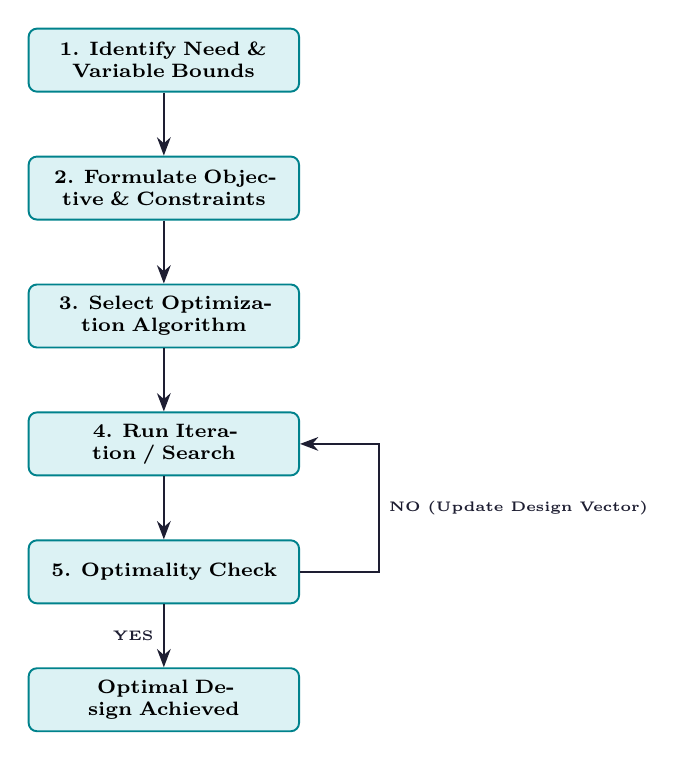
\begin{tikzpicture}[
  node distance=0.8cm and 1.5cm,
  block/.style={rectangle, draw=myteal, fill=hdrteal, text width=3.2cm, align=center, minimum height=0.8cm, font=\scriptsize\bfseries, rounded corners=3pt, line width=0.7pt},
  arrow/.style={-Stealth, thick, color=mydark}
]
  \node[block] (s1) {1. Identify Need \& Variable Bounds};
  \node[block, below=of s1] (s2) {2. Formulate Objective \& Constraints};
  \node[block, below=of s2] (s3) {3. Select Optimization Algorithm};
  \node[block, below=of s3] (s4) {4. Run Iteration / Search};
  \node[block, below=of s4] (s5) {5. Optimality Check};
  \node[block, below=of s5] (s6) {Optimal Design Achieved};

  \draw[arrow] (s1) -- (s2);
  \draw[arrow] (s2) -- (s3);
  \draw[arrow] (s3) -- (s4);
  \draw[arrow] (s4) -- (s5);
  \draw[arrow] (s5) -- node[left, font=\tiny\bfseries\color{mygreen}] {YES} (s6);
  
  \draw[arrow] (s5.east) -- ++(1.0,0) |- node[pos=0.25, right, font=\tiny\bfseries\color{myred}] {NO (Update Design Vector)} (s4.east);
\end{tikzpicture}
\end{tcolorbox}

\newpage

% ===============================================================================
% MANDATORY QUICK REVISION PAGE
% ===============================================================================
\begin{center}
  {\large\bfseries\color{myred} Quick Revision --- Module 1}\\[3pt]
  {\small\color{mydark} Mathematical Formulation \& Fundamentals $|$ OE-EC704B}
\end{center}
\noindent{\color{myred}\rule{\linewidth}{1.2pt}}
\vspace{4pt}

\begin{tcolorbox}[formulabox, title={\textbf{Key Concepts \& Mathematical Rules}}]
\renewcommand{\arraystretch}{1.35}
\begin{tabularx}{\linewidth}{B{5.0cm} X}
Objective Function & $f(\mathbf{x}) \rightarrow$ function to be minimized or maximized. \\[4pt]
Inequality Constraints & $g_j(\mathbf{x}) \le 0, \quad j=1,\dots,m$. \\[4pt]
Equality Constraints & $h_k(\mathbf{x}) = 0, \quad k=1,\dots,p$. \\[4pt]
Side Constraints & $x_i^{(L)} \le x_i \le x_i^{(U)}, \quad i=1,\dots,n$. \\[4pt]
Design Vector & $\mathbf{x} = [x_1, x_2, \dots, x_n]^T$ containing $n$ design variables. \\
\end{tabularx}
\end{tcolorbox}

\begin{tcolorbox}[defbox, title={\textbf{One-Line Definitions}}]
\begin{itemize}[leftmargin=*, itemsep=2.5pt, topsep=0pt]
  \item \textbf{Design Variable:} An independent parameter that can be varied during the design optimization process.
  \item \textbf{Behavior Constraint:} A constraint bounding the system behavior under operational loads (e.g., maximum stress).
  \item \textbf{Feasible Space:} The region of design space in which all inequality and equality constraints are fully satisfied.
  \item \textbf{Non-linear Programming (NLP):} An optimization problem containing non-linearities in objective or constraint functions.
  \item \textbf{Global Minimum:} The absolute lowest value of the objective function in the entire feasible design space.
  \item \textbf{Local Minimum:} The lowest value of the objective function within a local neighborhood of the design space.
\end{itemize}
\end{tcolorbox}

\begin{tcolorbox}[exambox, title={\textbf{Frequently Asked / Viva Questions}}]
\begin{enumerate}[topsep=0pt, label=\textbf{Q\arabic*.}, itemsep=5pt]
  \item \Q{State the standard mathematical formulation of a constrained optimization problem.}
    Minimize $f(\mathbf{x})$ subject to $g_j(\mathbf{x}) \le 0$ for $j=1,\dots,m$, $h_k(\mathbf{x}) = 0$ for $k=1,\dots,p$, and $x_i^{(L)} \le x_i \le x_i^{(U)}$ for $i=1,\dots,n$.
  \item \Q{Differentiate between design variables and design parameters.}
    Design variables are changed by the optimization algorithm to find the optimum design. Design parameters are constant coefficients fixed before the optimization starts (e.g., material density, young's modulus).
  \item \Q{Differentiate between behavior constraints and side constraints.}
    Behavior constraints depend on the state variables of the system and require system analysis to evaluate (e.g., stress $\le \sigma_{allow}$). Side constraints directly bound the design variables (e.g., diameter $d \ge 10\text{ mm}$).
  \item \Q{What is a feasible design space?}
    A feasible design space is the collection of all design vectors $\mathbf{x}$ that satisfy all constraints simultaneously.
  \item \Q{What is the difference between single-objective and multi-objective optimization?}
    Single-objective optimization seeks to optimize a single criterion. Multi-objective optimization optimizes multiple conflicting objectives simultaneously, yielding a set of trade-off designs (Pareto front).
  \item \Q{Why do we reformulate a maximization problem as a minimization problem?}
    To maintain algorithmic consistency. Any maximization problem can be solved using standard minimization algorithms by minimizing $-f(\mathbf{x})$.
  \item \Q{What makes a problem a Linear Programming Problem (LPP)?}
    An optimization problem is an LPP if the objective function and all equality/inequality constraints are linear functions of the design variables.
  \item \Q{Classify optimization methods based on their search logic.}
    Methods are classified into Analytical Methods (calculus-based), Numerical Methods (Search-based: Direct and Gradient-based), and Advanced Heuristic Methods (nature-inspired: GA, PSO, SA).
  \item \Q{Explain the role of the objective function.}
    The objective function acts as a mathematical evaluator that measures how good a particular candidate design vector is relative to design goals.
  \item \Q{What are the side constraints in cylinder volume maximization under surface area limits?}
    The side constraints are the physical non-negativity limits of the geometric parameters: Radius $r \ge 0$ and Height $h \ge 0$.
\end{enumerate}
\end{tcolorbox}

\end{document}
